\chapter{実際の動作しているサイト}

現在、下記レポジトリ、サイトで実際に動作しています。
実際にesaから記事を取り出して、GitHubにpushしているので、記事を更新するだけで、Webサイトが更新されます。


レポジトリ:
\url{https://github.com/SystemEngineeringTeam/BlogSiteMarkDown}

Webサイト:
\url{https://esa.harutiro.net/}

\begin{figure}[htbp]
  \begin{minipage}{0.5\hsize}
      \begin{center}
          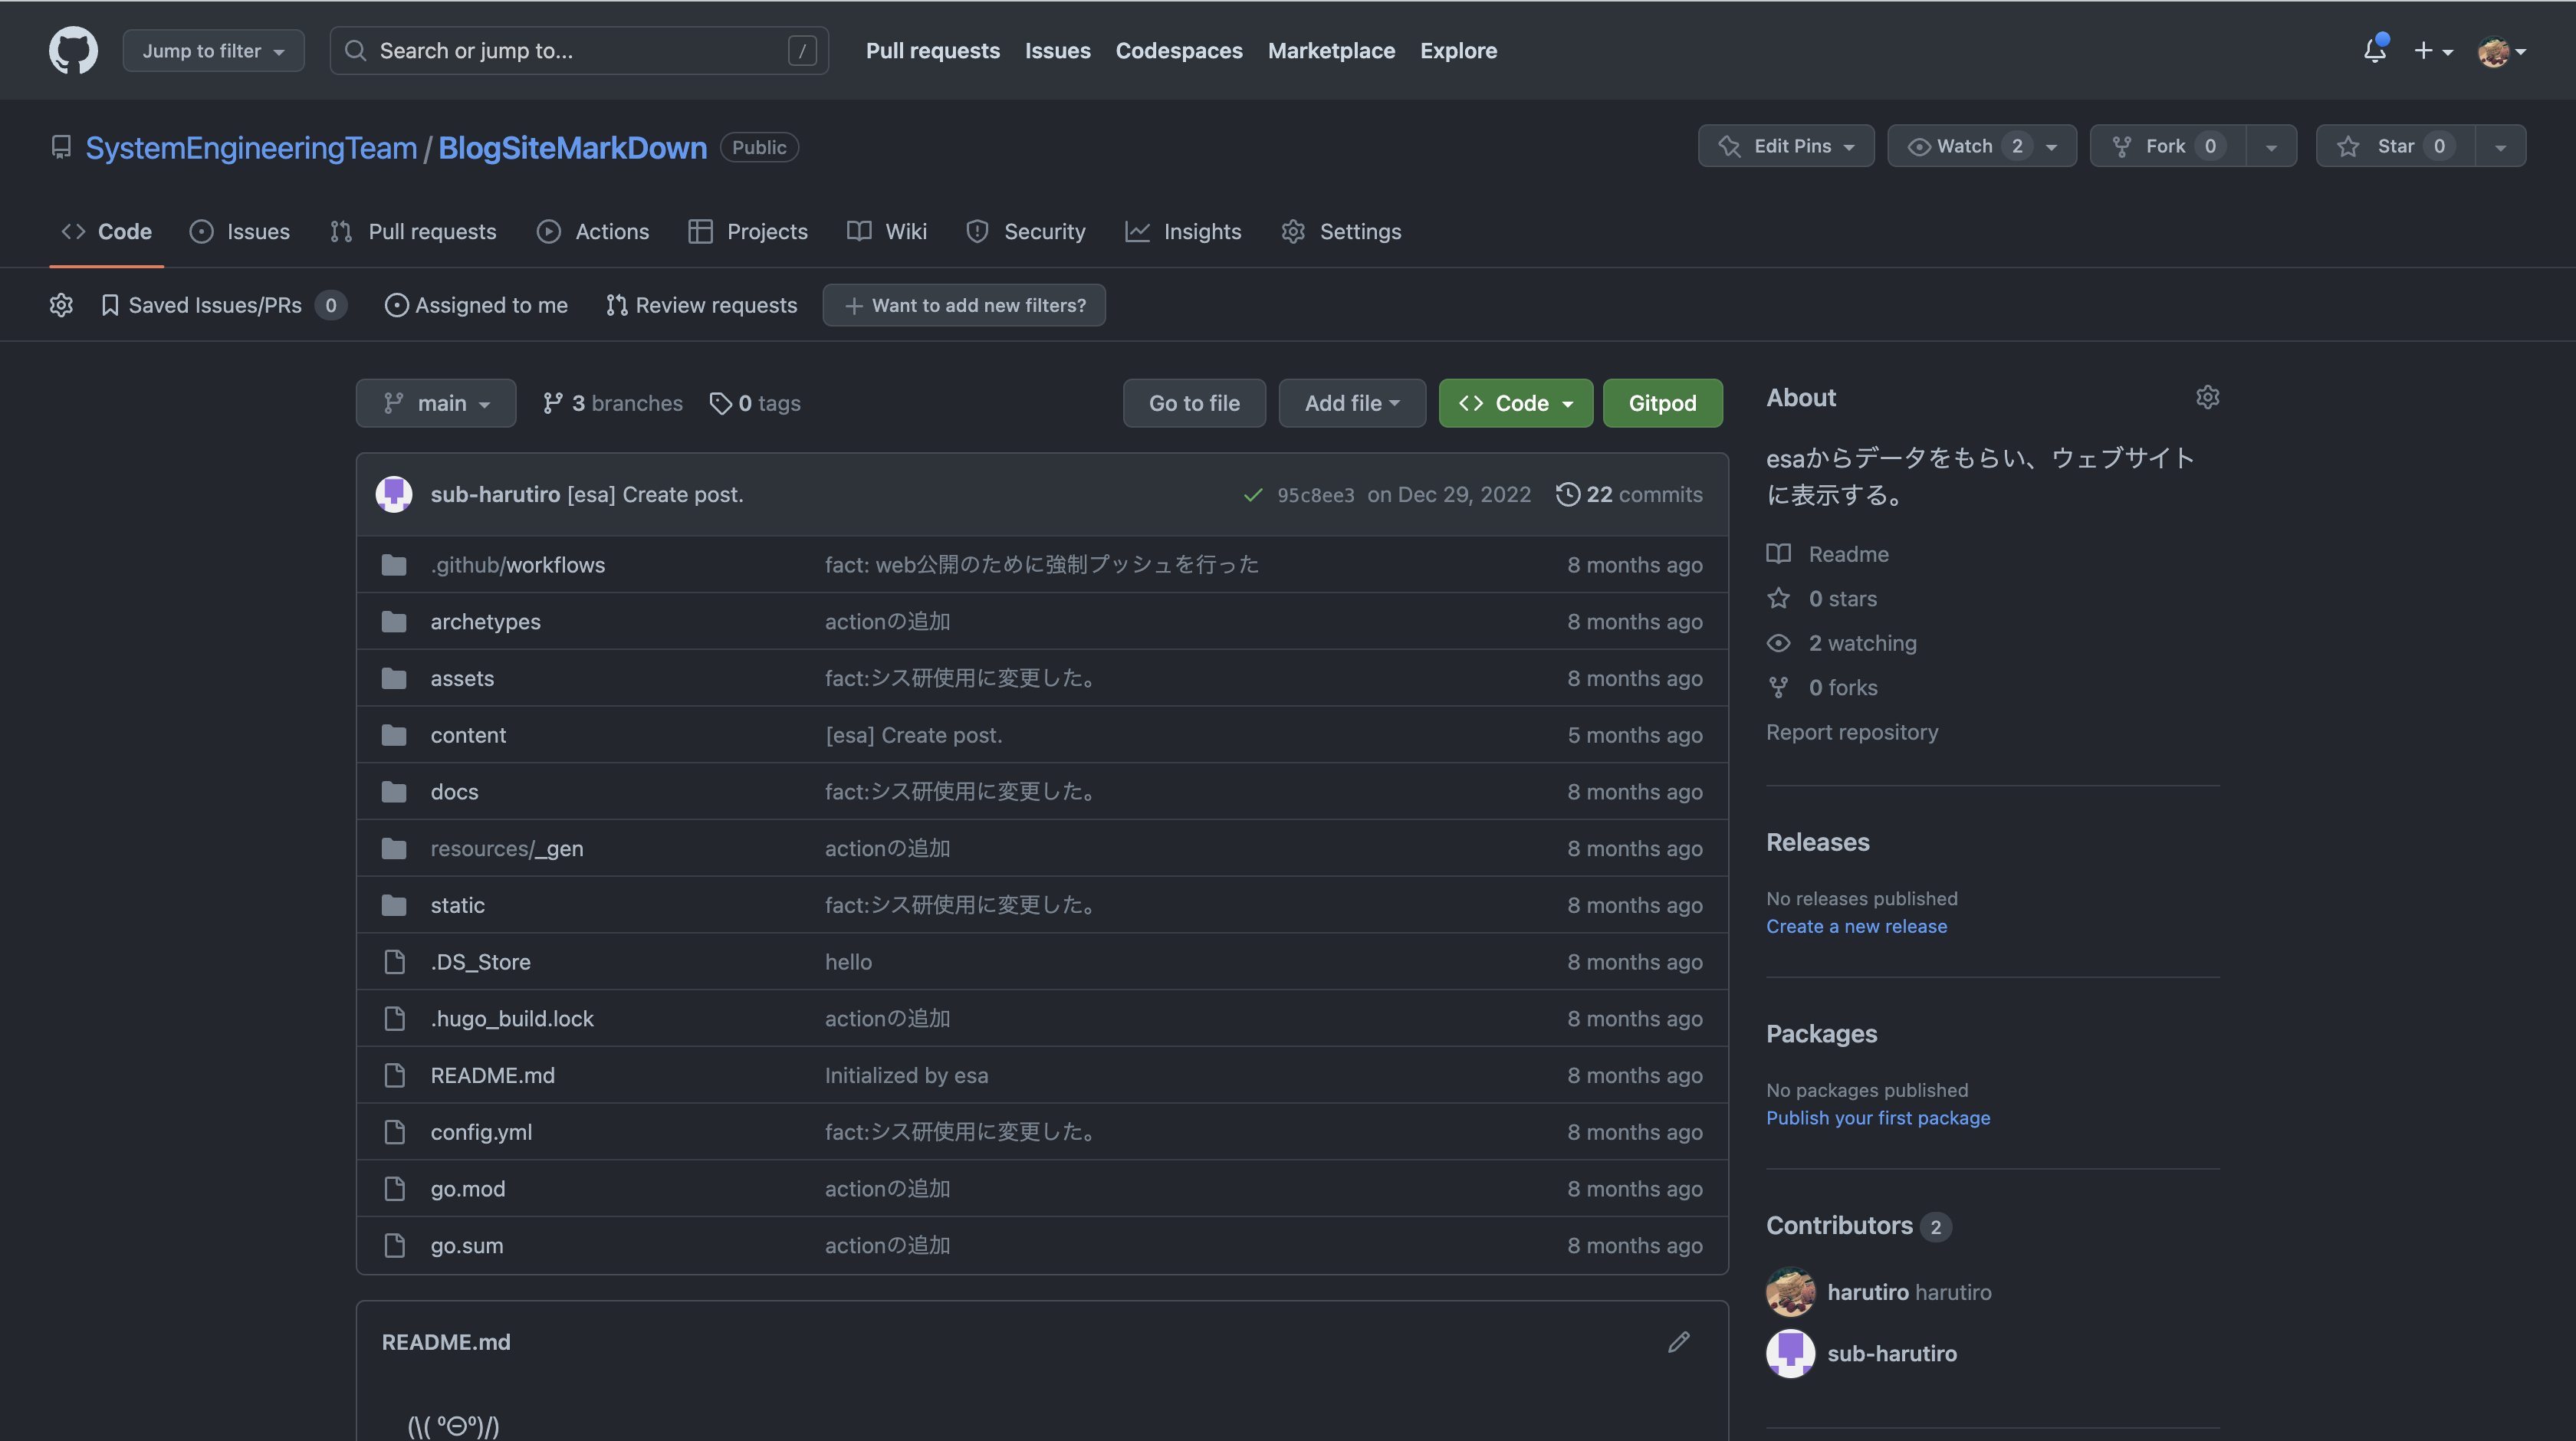
\includegraphics[width=50mm]{./image/02-chap2/git-repo.png}
      \end{center}
      \caption{Gitレポジトリ}
      \label{chap2-git-repo}
  \end{minipage}
  \begin{minipage}{0.5\hsize}
      \begin{center}
          
\includegraphics[width=50mm]{./image/02-chap2/sysken-web.png}
      \end{center}
      \caption{Webサイト}
      \label{chap2-web-site}
  \end{minipage}
\end{figure}